\documentclass[12pt]{cheatsheet}
\usepackage{blindtext}
\usepackage{enumitem}
\setlist{itemsep=0.2em, topsep=0.2em}
\usepackage{amsmath}
\usepackage{xcolor}
\usepackage{cancel}
\usepackage{tikz}
\usetikzlibrary{arrows.meta, positioning, shapes}

\author{Gian Maria Ernst - ernstg\\  \vspace*{0.2em} \vspace*{-0.2em}}\doctitle{Bioengineering}

\begin{document}
\small
\scalebox{0.7}{
\begin{tabular}{@{}lcc@{}}

Tera   & T      & $10^{12}$ \\
Giga   & G      & $10^{9}$ \\
Mega   & M      & $10^{6}$ \\
\end{tabular}
}
\scalebox{0.7}{
\begin{tabular}{@{}lcc@{}}
    Kilo   & k      & $10^{3}$ \\
    
    Milli  & m      & $10^{-3}$ \\
Mikro  & $\mu$  & $10^{-6}$ \\
\end{tabular}
}
\scalebox{0.7}{
\begin{tabular}{@{}lcc@{}}
Nano   & n      & $10^{-9}$ \\
Piko   & p      & $10^{-12}$ \\
Femto  & f      & $10^{-15}$ \\
\end{tabular}
}


\section*{Orientation of the cell}
Central Dogma of Molecular Biology
\[
\boxed{
    \begin{aligned}
        \text{DNA} \ &\xrightarrow{\text{transcription}} \text{mRNA} \xrightarrow{\text{translation}} \text{proteins}
    \end{aligned}
}
\]
Cells:\\
\includegraphics[width=7.3cm]{src/images/cell.png}

\begin{minipage}{0.45\linewidth}
    \includegraphics[width=3cm]{src/images/organelles.png}
\end{minipage}
\begin{minipage}{0.55\linewidth}
    \textbf{nucleus}: houses DNA for EK\\
    \textbf{nucleolus}: produces ribosomes/rRNA\\
    \textbf{mitochondria}: cellular respiration (prod. ATP)\\
    \textbf{ribosome}: produces proteins from mRNA transcripts\\
    
\end{minipage}
\vspace{1mm}
\textbf{RER, SER and Golgi}: involved in protein/lipid synthesis/processing\\
\textbf{cytoskeleton}: structure to cell, transport mol. in the cell or to enable the cell to move (cell migration)\\
\textbf{centrosome}: organizes microtubules during cell division allows the mother cell to split into 2 cells\\


\section*{Building Blocks}
\begin{minipage}{0.4\linewidth}
    Cell composition:\\
    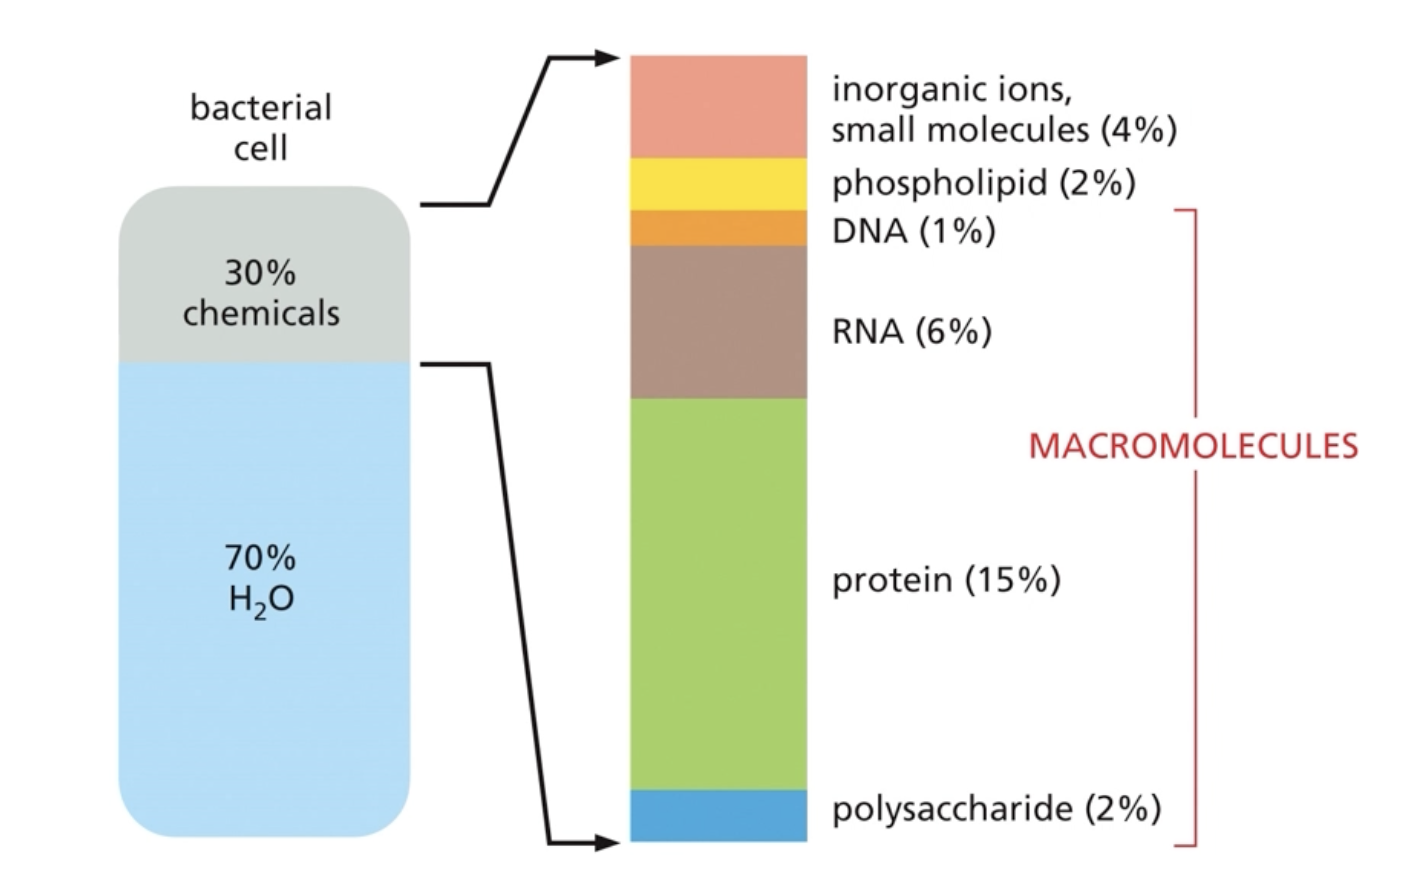
\includegraphics[width=3cm]{src/images/cell_composition.png}
\end{minipage}
\begin{minipage}{0.45\linewidth}
    Main building blocks:\\
    \vspace{1mm}
    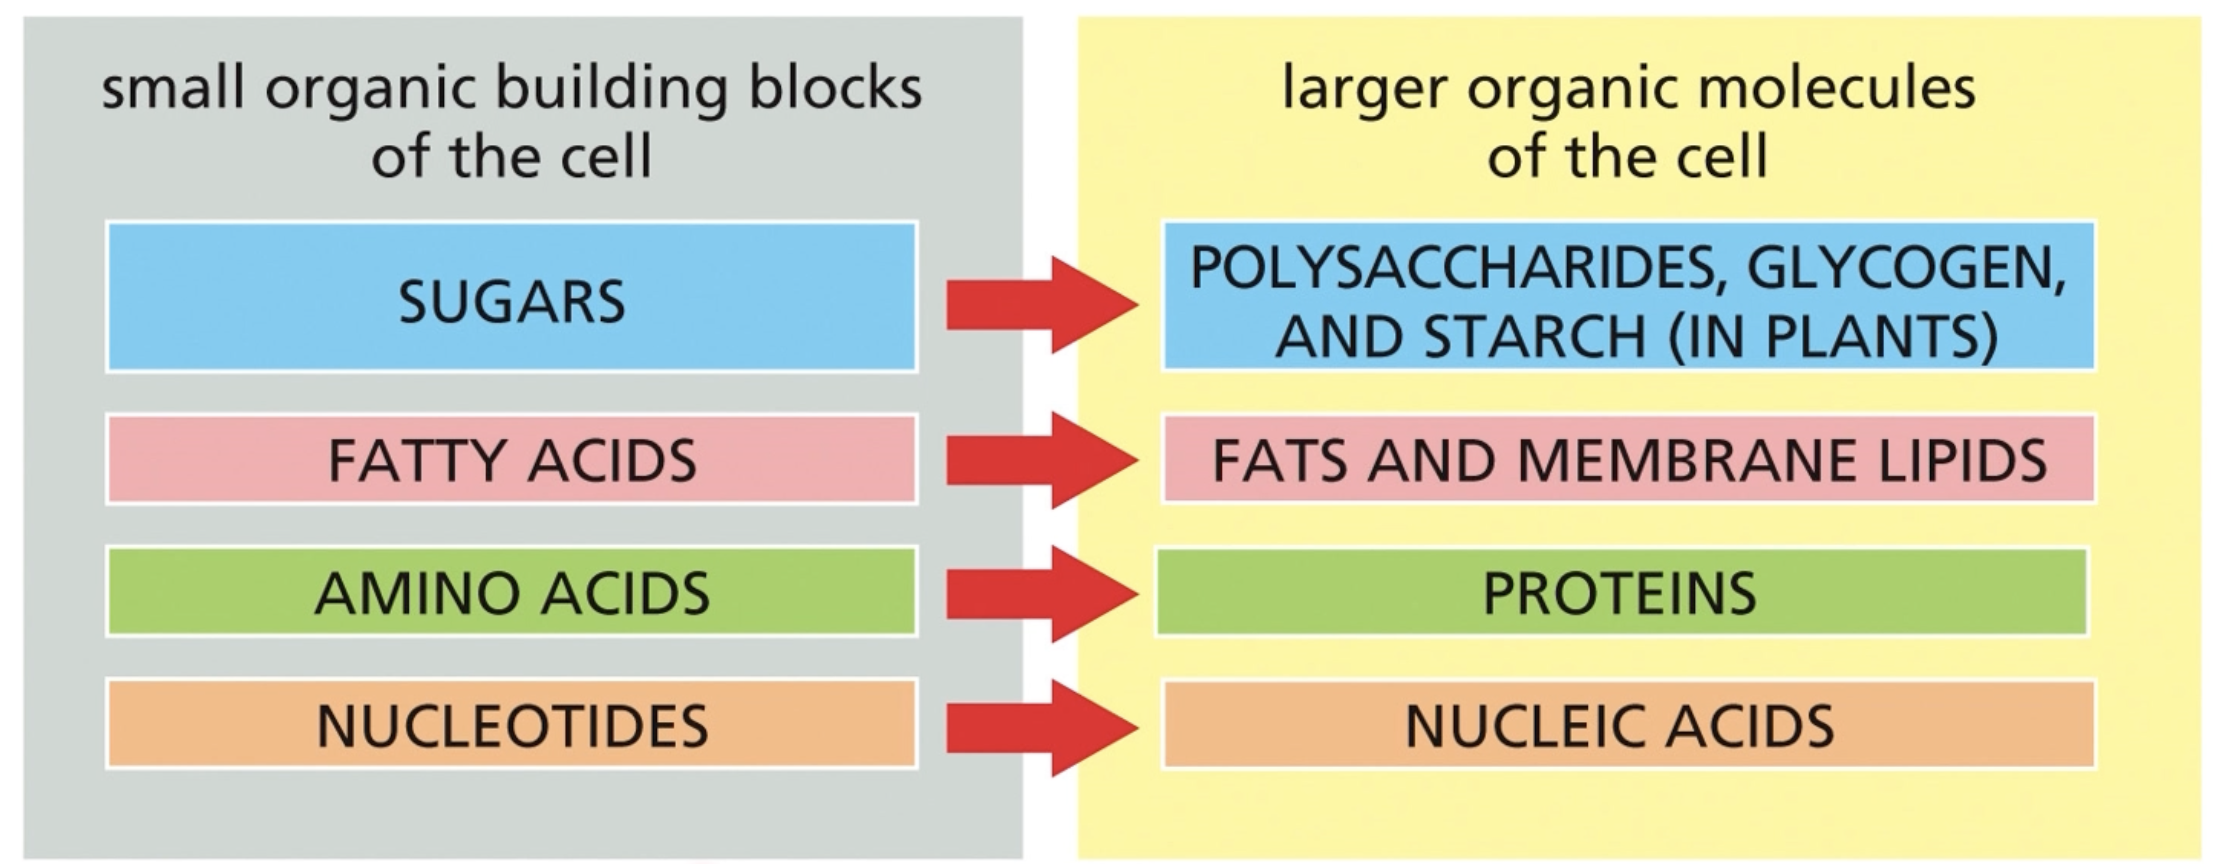
\includegraphics[width=4cm]{src/images/main_building_blocks.png}
\end{minipage}  

\begin{itemize}
\item \textbf{Lipids} (fatty acids): long-term energy storage, cell membrane structure, signaling molecules.
\item\textbf{Proteins} (amino acids): perform most of the cell's functions, including catalyzing reactions, signaling, and structural support.
\hspace{11mm} amino group $\textbf{NH}_2$, carboxyl group \textbf{COOH}
\item \textbf{Nucleic acids} (nucleotides): store and transmit genetic information (DNA, RNA), carry energy
\item \textbf{Carbohydrates} (Sugars): short-term energy storages and for structural support.
\end{itemize}
    

\subsection*{Bounds}
\begin{minipage}{0.5\linewidth}
    \[
    \boxed{        
            K_D = \frac{k_{off}}{k_{on}}
    }
    \]
\end{minipage}\begin{minipage}{0.4\linewidth}
\begin{align*}
    \text{Covalent} &\longleftrightarrow 100 k_B T\\
    \text{Ionic} &\longleftrightarrow 1-10 k_B T\\
    \text{Hydrogen} &\longleftrightarrow 1 k_B T\\
    \text{Van der Waals} &\longleftrightarrow 0.1 k_B T\\
    \text{Electrostatic} &\longleftrightarrow 0.1 k_B T
\end{align*}
\end{minipage} 

    $K_D$: Equilibrium constant\\
    indicates the ratio of free \& bound units\\
    $k_{off}$: Dissociation rate constant\\
    inverse of time protein dissociates from the ligand\\
    $k_{on}$: Association rate constant, speed of the reaction



%\vfill \null \columnbreak
\subsection*{Enzymes (aka catalysts)}
\begin{itemize}
\item Accellerate reaction by lowering the activation energy
\item Are not consumed in the reaction
\item Are specific to the reaction they catalyze
\item Do not change the equilibrium point of the reaction.
\end{itemize}

\section*{Energy and Metabolism}
\begin{minipage}{0.5\linewidth}
   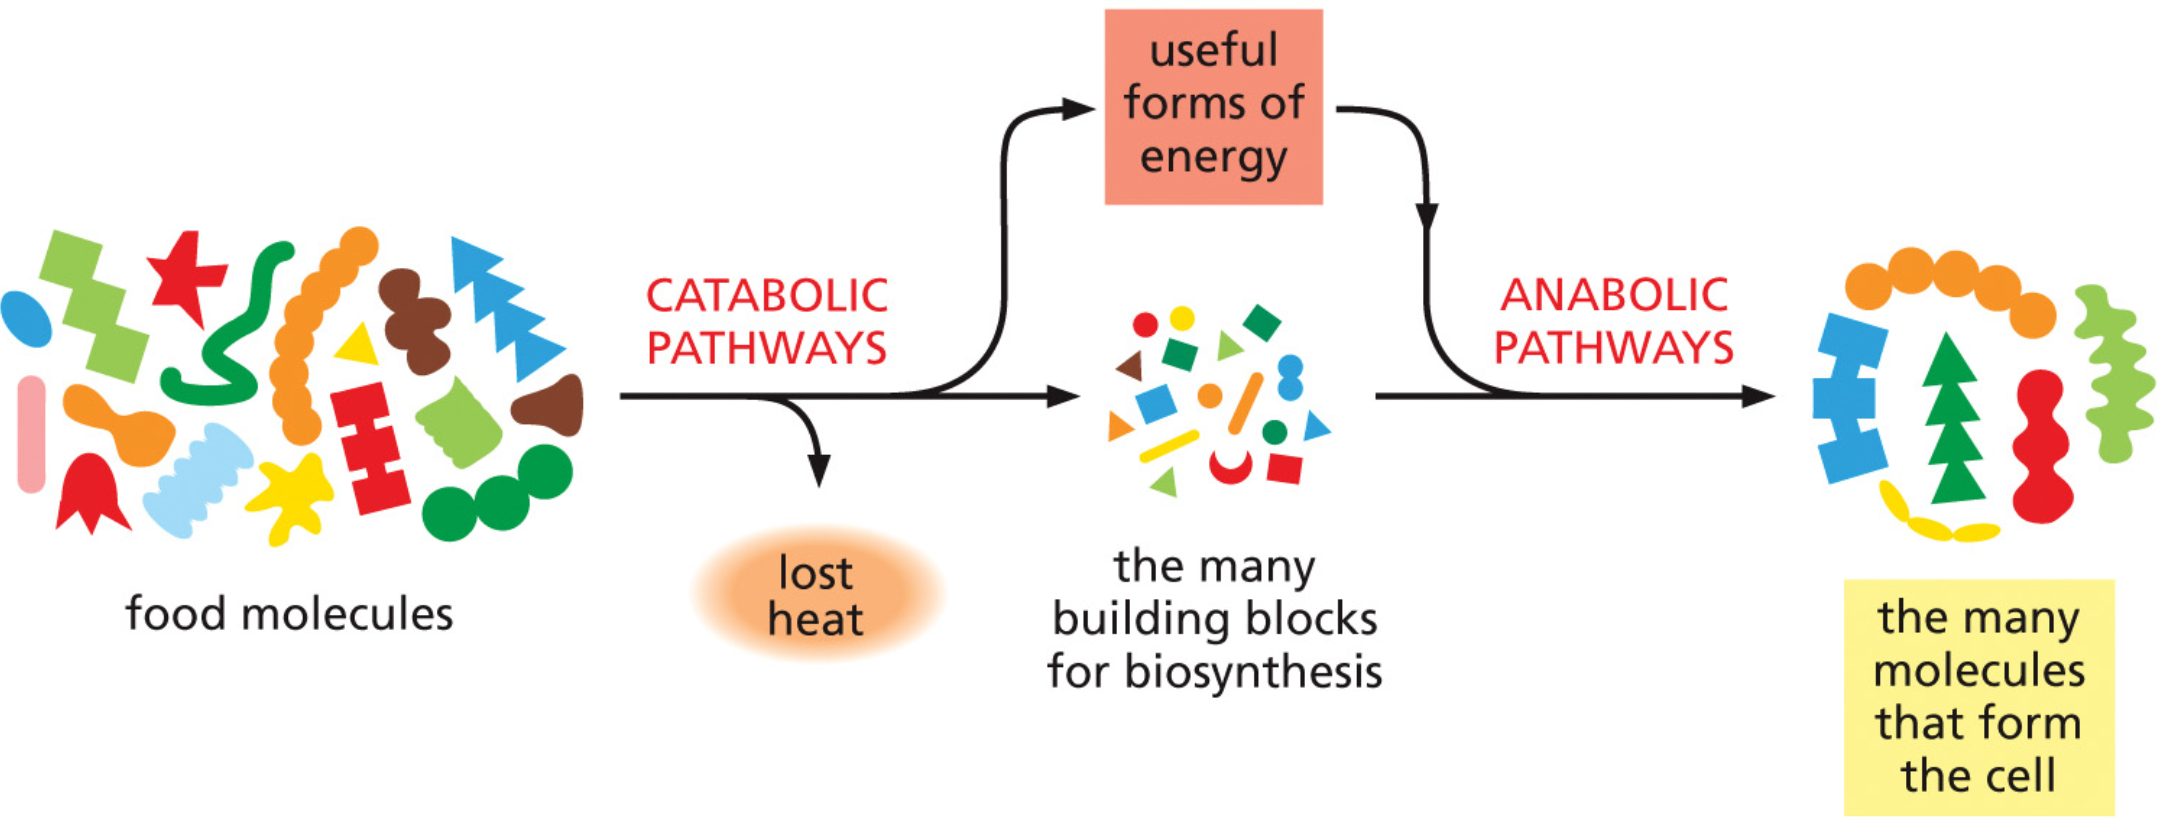
\includegraphics[width=4cm]{src/images/energy_matter.png} 
\end{minipage}
\begin{minipage}{0.5\linewidth}
    \begin{itemize}
\item \textbf{Catabolism:} Breakdown (glycolysis, citric acid cycle)
\item \textbf{Anabolism:} Synthesis (protein synthesis, DNA replication)
\end{itemize}
\end{minipage}
\subsection*{Free Energy}
\begin{minipage}{0.2\linewidth}
        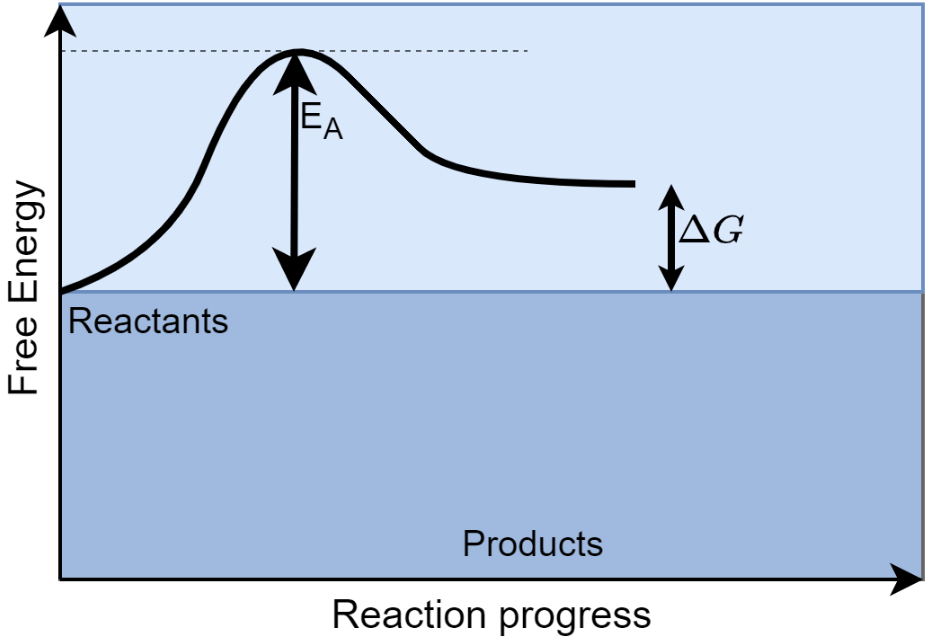
\includegraphics[width=15mm]{src/images/Endergonic.png}\\ 
\end{minipage}
\begin{minipage}{0.28\linewidth}
    $\Delta G > 0$\\
    Endergonic\\
    requires energy\\
    not spontaneously\\
\end{minipage}
\begin{minipage}{0.2\linewidth}
        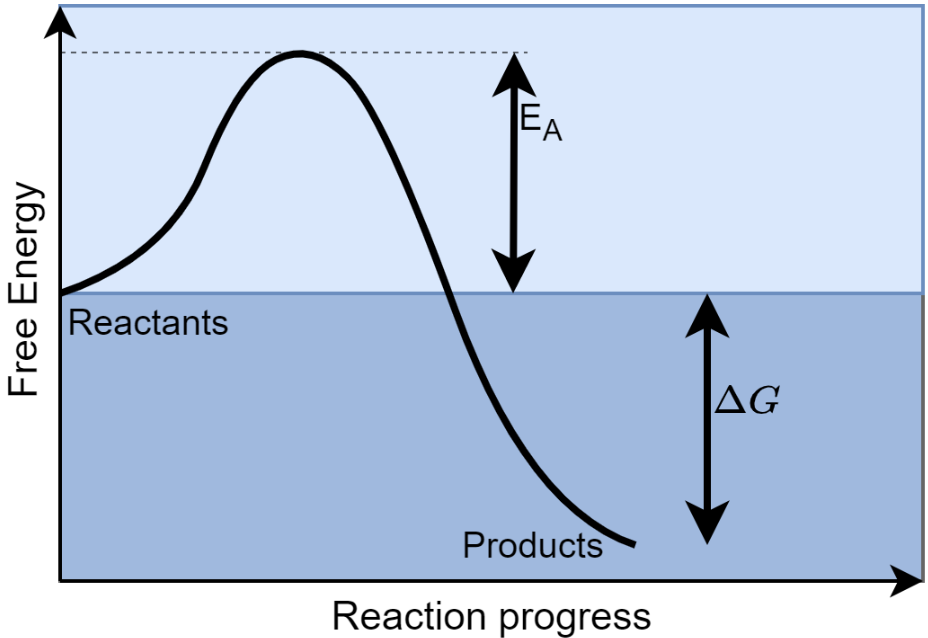
\includegraphics[width=15mm]{src/images/Exergonic.png}\\ 
\end{minipage}
\begin{minipage}{0.28\linewidth}
    $\Delta G < 0$\\
    Exergonic\\
    releases energy\\
    spontaneously\\
\end{minipage}



\subsection*{Redox}
Oxidation loss of $e^-$ ($H^+ + e^-$) $\vert$ Oxidation of glucose \\
Reduction gain of $e^-$ ($H^+ + e^-$)$\vert$ Reduction of pyruvate\\

$\text{NADH}\rightleftharpoons \text{NAD}^+ + 2e^- + H^+$ $\vert$ $\rightharpoonup$ oxidation, $\leftharpoondown$ reduction

\subsection*{Glucose Metabolism}
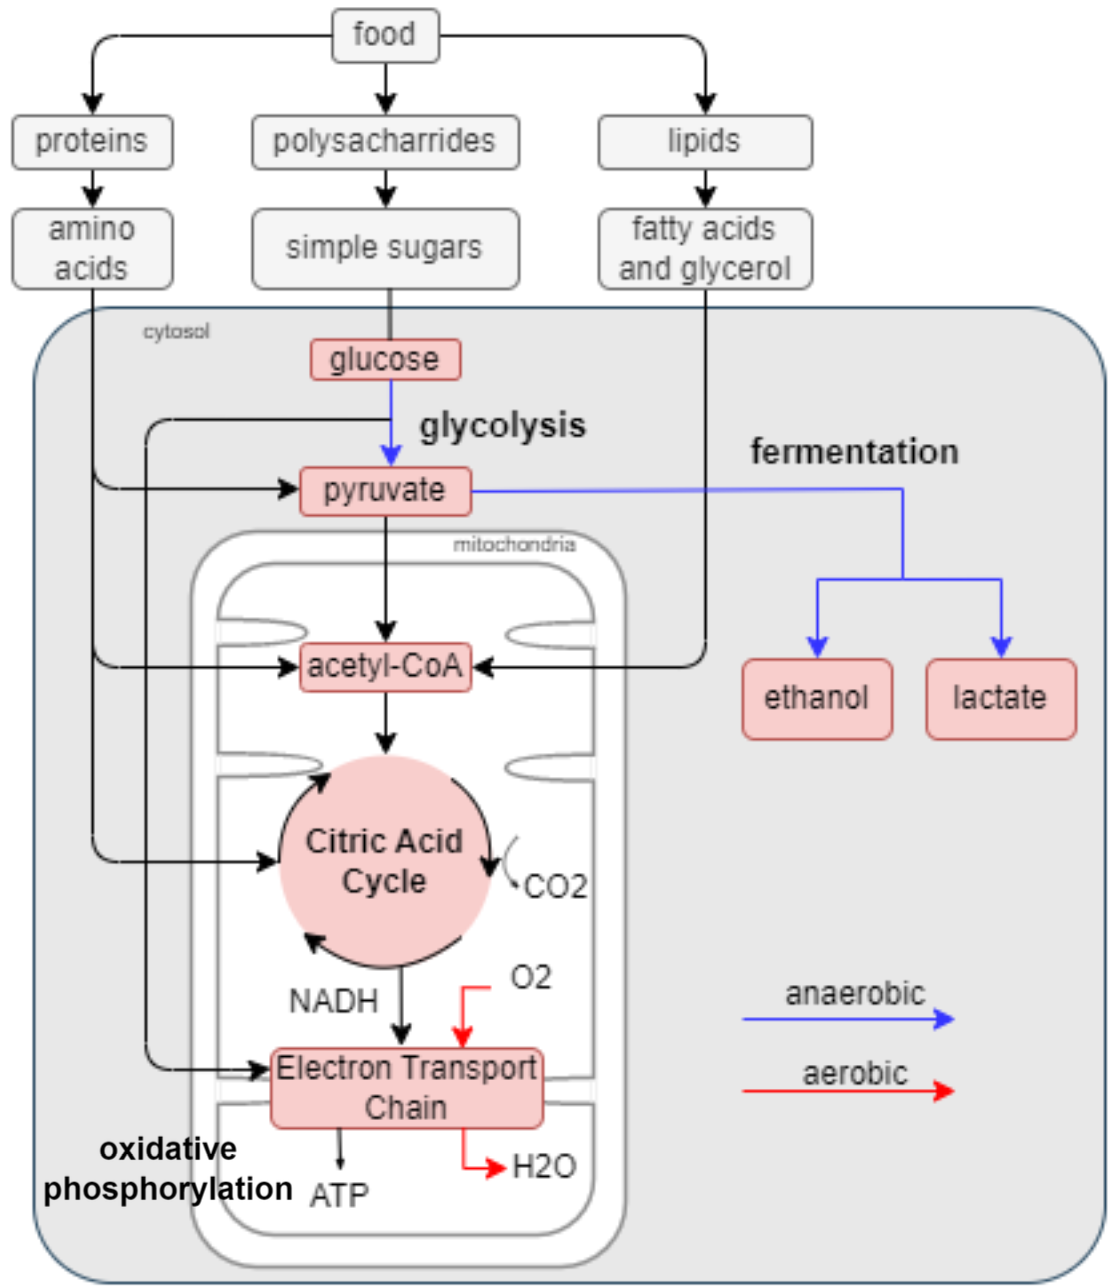
\includegraphics[width=7cm]{src/Images/glucose_metabolism.png}\\ 

\begin{tabular}{l p{5cm}}
\textbf{Stage} & \textbf{Molecules} \hfill \textbf{Glycolysis}\\
\hline
Invest   & 2 ATP, 2 NAD\(^+\), 1 glucose \\
Payoff   & 4 ATP (2 net), 2 NADH, 2 H\(^+\), 2 pyruvate \\
Net gain & 2 ATP, 2 NADH, 2 pyruvate \\
\hline
\end{tabular}
\begin{tabular}{l p{5cm}}
\textbf{Stage} & \textbf{Molecules} \hfill \textbf{Citric Acid Cycle}\\
\hline
Invest   & 2 Acetyl-CoA, 6 NAD\(^+\), 2 FAD, 2 GDP (ADP) \\
Payoff   & 6 NADH, 2 FADH\(_2\), 2 GTP (ATP), 4 CO\(_2\) \\
Net gain & 2 ATP (GTP), 6 NADH, 2 FADH\(_2\), 4 CO\(_2\) \\
\hline
\end{tabular}
\begin{tabular}{l p{5cm}}
\textbf{Stage} & \textbf{Molecules} \hfill \textbf{Oxidative Phosphorylation}\\
Invest   & 10 NADH, 2 FADH\(_2\), 6 O\(_2\) \\
Payoff   & 34 ATP, 6 H\(_2\)O \\
Net gain & 34 ATP, 6 H\(_2\)O \\
\hline
\end{tabular}\\


\section*{Biosynthesis}
\begin{minipage}{0.38\linewidth}
    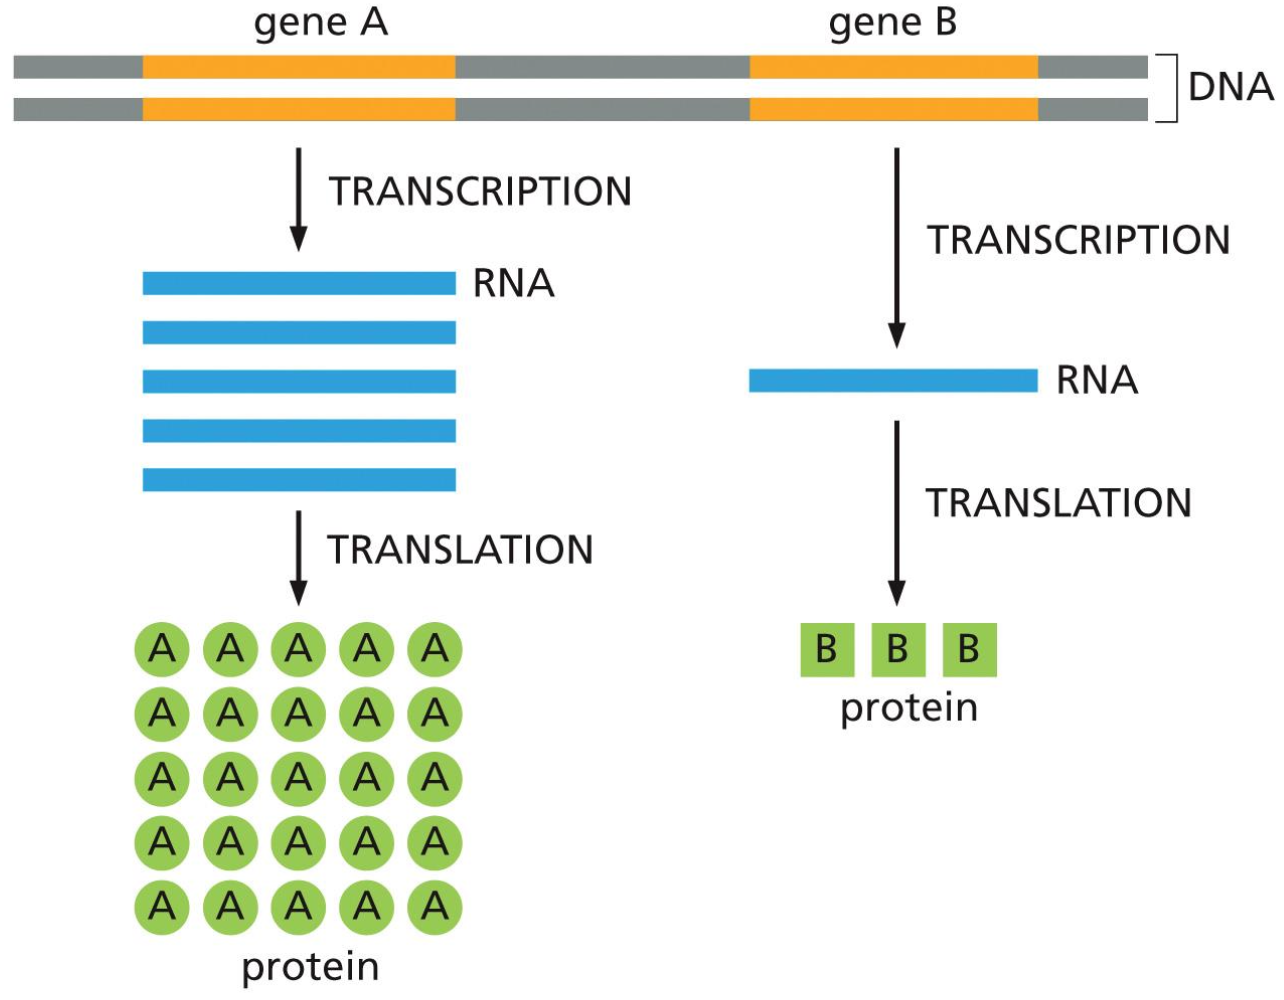
\includegraphics[width=25mm]{src/Images/biosynthesis_of_protein.png}\\ 
\end{minipage}
\begin{minipage}{0.62\linewidth}
Genes are not always on and do not always produce the same number of transcripts or proteins.\\

Synthesis of proteins is a complicated and tightly regulated process.
\end{minipage}



\subsection*{Transcription}
\begin{minipage}{0.32\linewidth}
    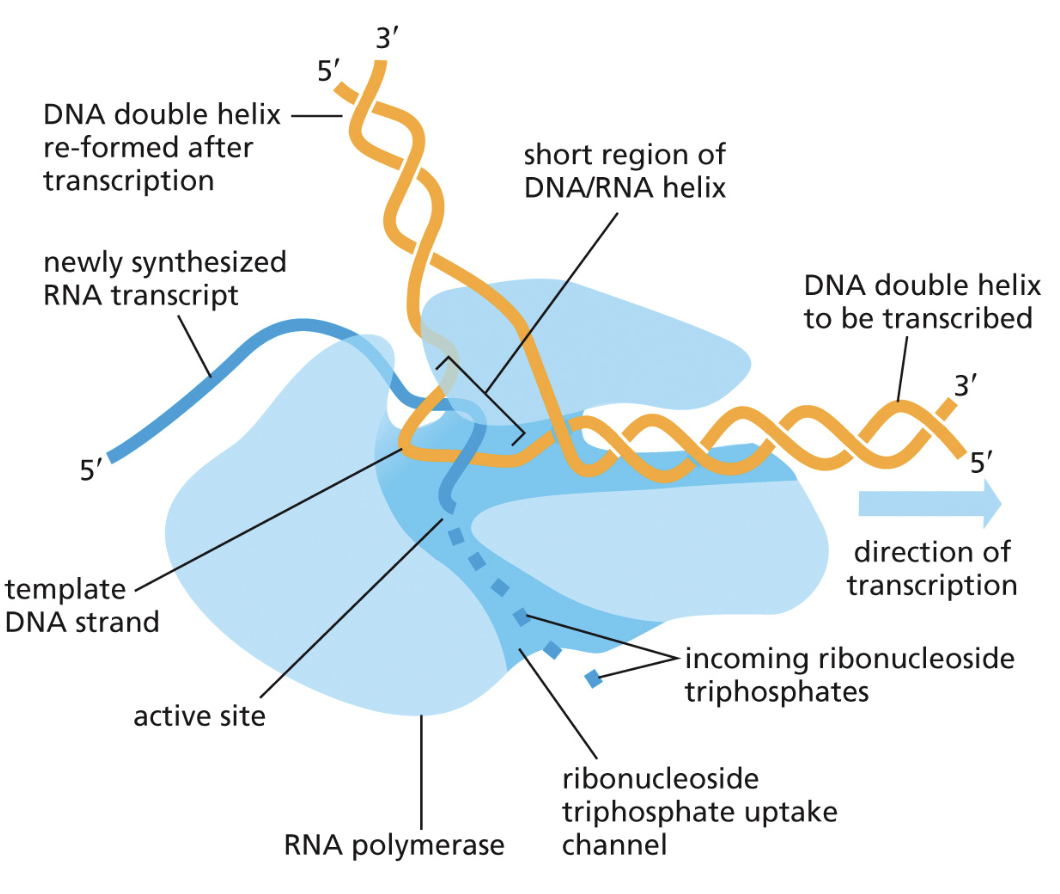
\includegraphics[width=28mm]{src/Images/transcription.png}\\ 
\end{minipage}
\begin{minipage}{0.68\linewidth}
\begin{enumerate}
    \item Small region of DNA opens and unwinds.
    \item RNA polymerase (catalytic enzyme) interacts with one strand in the open region of DNA and adds ribonucleotides to grow an RNA polymer.
    \item RNA polymerase further unwinds the DNA in the forward direction.
\end{enumerate}
\end{minipage}
\subsection*{types of RNA}
\begin{tabular}{l p{38mm}}
\textbf{Type } & \textbf{Function} \\
\hline
messenger RNA \textbf{mRNA}   & code for proteins \\
ribosomal RNA \textbf{rRNA}   & form core of ribosom structure and catalize protein synthesis \\
micro RNA \textbf{miRNA} & regulate gene expression\\
transfer RNA \textbf{tRNA} & serve as adaptors between mRNA and amino acids during protein synthesis \\
other non-coding RNA & RNA splicing, gene regulation, telomere maintenance, etc. \\
\end{tabular}\\
\subsection*{Eukaryotes vs Prokaryotes}

\begin{minipage}{0.32\linewidth}
    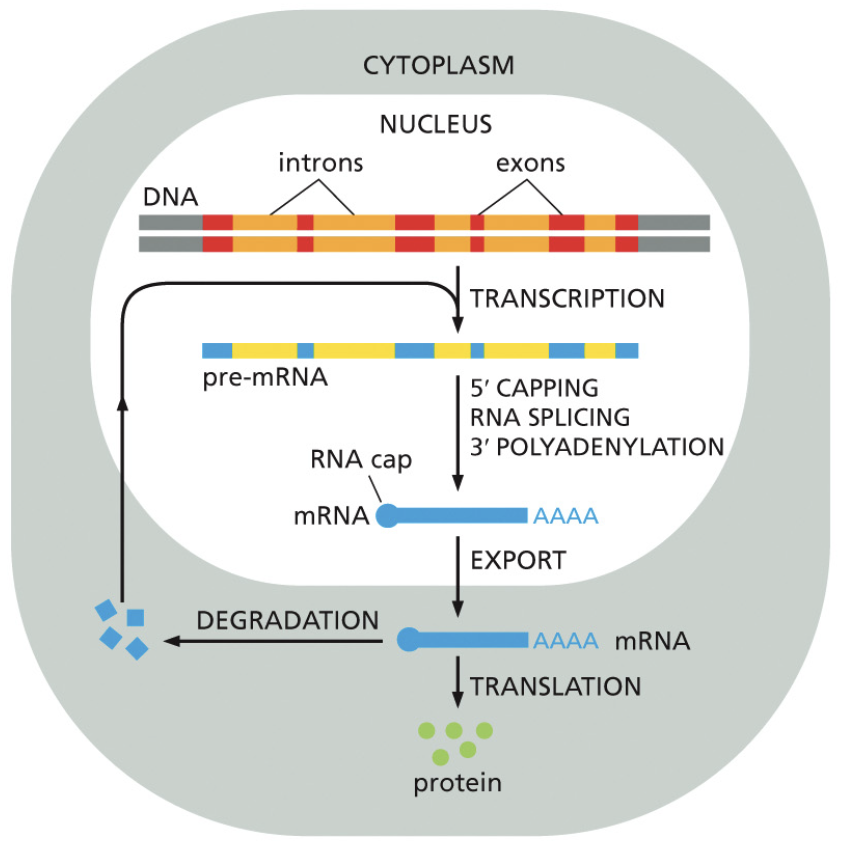
\includegraphics[width=28mm]{src/Images/eukaryot_transcription.png}\\ 
\end{minipage}
\begin{minipage}{0.68\linewidth}
\begin{itemize}
    \item Multiple types of RNA polymerases transcribe different classes of RNA.
    \item Transcription initiation is more complex.
    \item mRNA molecules undergo splicing, where introns (non-coding regions) are removed and exons (coding regions) are joined together to form the final RNA.
\end{itemize}
\end{minipage}
\hrule
\vspace{2mm}
\begin{minipage}{0.32\linewidth}
    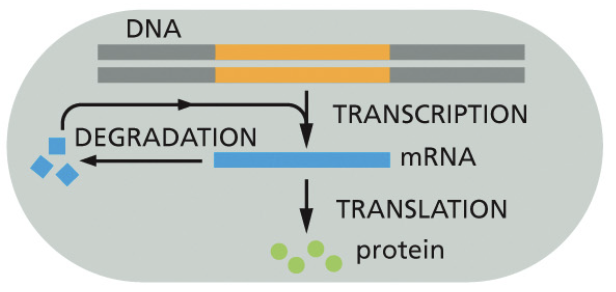
\includegraphics[width=28mm]{src/Images/prokaryot_transcription.png}\\ 
\end{minipage}
\begin{minipage}{0.68\linewidth}
\begin{itemize}
    \item 1 type of RNA polymerase transcribes all types of RNA.
    \item Transcription initiation is a simpler process.
    \item mRNA molecules are translated immediately after
transcription
\end{itemize}
\end{minipage}
\hrule
\vspace{2mm}
Both use gene regulatory proteins that bind to
specific sequences of DNA:
\begin{itemize}
    \item Repressors: Bind to sequences to turn genes off. Make it more difficult for RNA polymerase to bind to DNA.
    \item Activators: Bind to sequences to turn genes on. Make it more favorable for RNA polymerase to bind to DNA.
\end{itemize}

\subsection*{Gene Regulation}
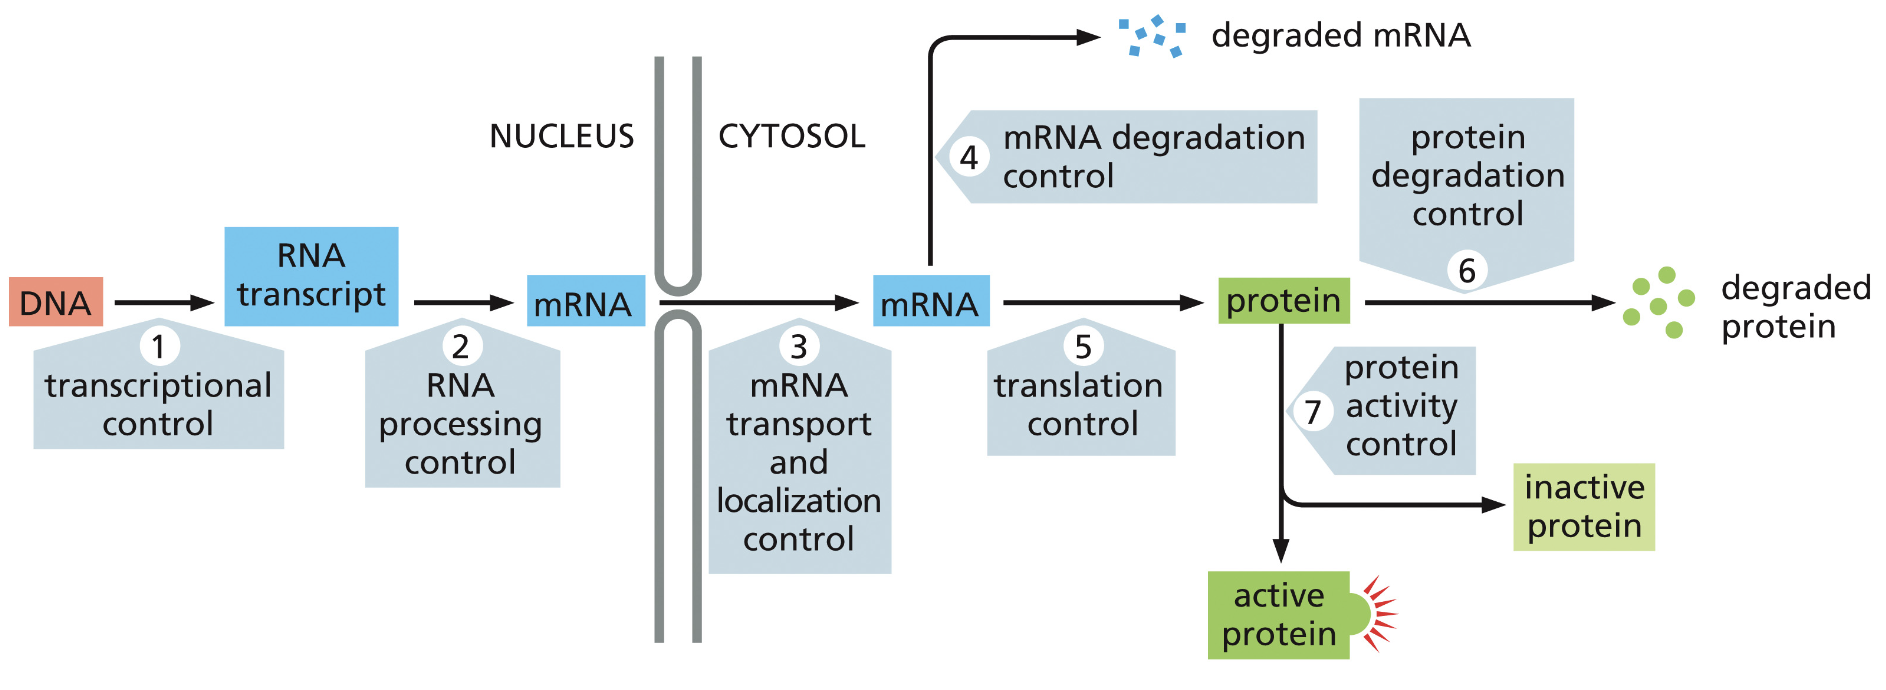
\includegraphics[width=70mm]{src/Images/gene_regulation.png}\\ 
\subsection*{Translation by Ribosomes}
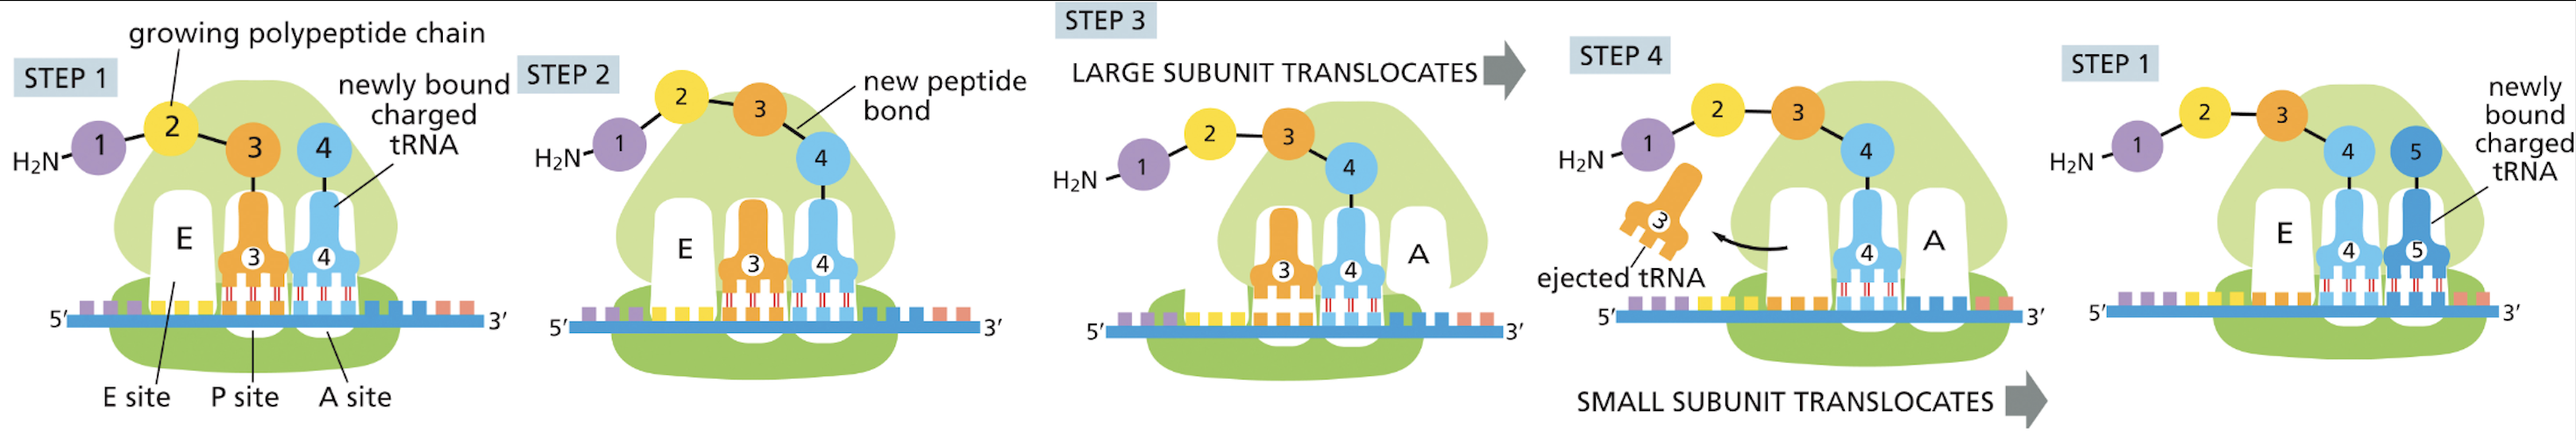
\includegraphics[width=70mm]{src/Images/translation_ribosome.png}\\ 
\begin{itemize}
    \item On the mRNA, every three bases (= nucleotides) form one codon (needs ATP).
    \item A tRNA brings a matching amino acid. It has an anticodon that is complementary to the mRNA codon.
    \item The tRNA binds to the mRNA in the ribosome (at the A site).
    \item The amino acid is added to the growing polypeptide chain.
    \item The tRNA is ejected (from the E site), and the ribosome shifts forward by one codon.
    \item The process repeats until a stop codon is reached.
\end{itemize}
Multiple ribosomes can translate the same mRNA at the same time (making multiple proteins at the time), forming a polyribosome (or polysome).









\section*{Transport and Exchange}
\subsection*{Cell Membrane}

\begin{minipage}{0.40\linewidth}
    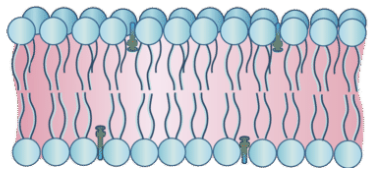
\includegraphics[width=28mm]{src/Images/cell_membrane.png}
\end{minipage}
\begin{minipage}{0.6\linewidth}
Phospholipid bilayer with hydrophilic head and hydrophobic tail act as barrier between compartements.\\
Only small nonpolar molecules can pass through the membrane.\\
\end{minipage}

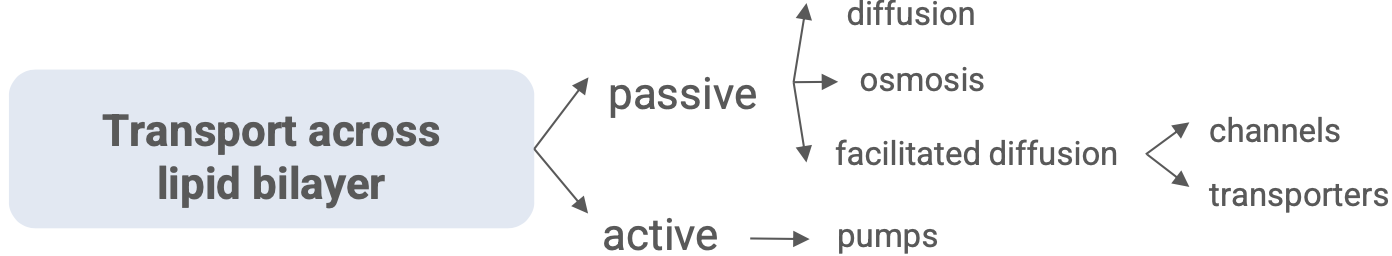
\includegraphics[width=70mm]{src/Images/transport_across_bilayer.png}


\subsection*{Passive Transport}

\begin{minipage}{0.5\linewidth}
    \textbf{Diffusion:}\\
    Along conzentration gradient, from high to low concentration.
        \[
    \boxed{        
            \tau_D = \frac{l^2}{(6)D} 
            \hspace{2mm}
            D = \frac{k_B T}{6 \pi \eta a}
    }
    \]
    \vspace{7mm}
\end{minipage}
\begin{minipage}{0.5\linewidth}
    \textbf{Osmosis:}\\
        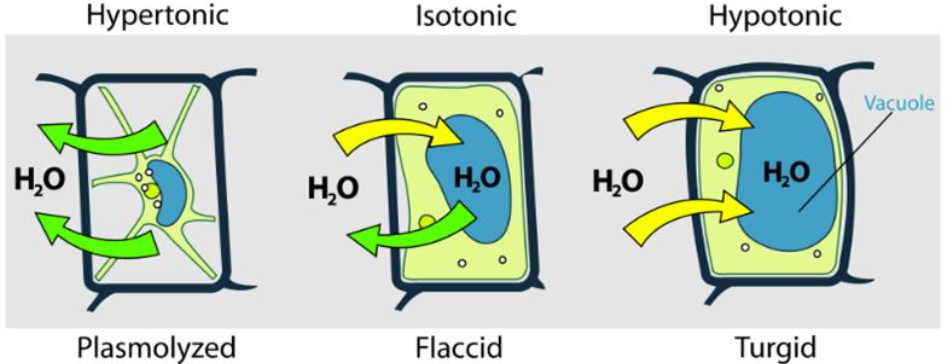
\includegraphics[width=35mm]{src/Images/osmosis.png}
        Hypertronic: high solute concentration\\
        Hypotonic: low solute concentration.\\
\end{minipage}

Membrane is \textbf{selectively permeable}, allowing some molecules to pass through while blocking others.\\

\textbf{Facilitated Diffusion:}\\
\begin{minipage}{0.42\linewidth}
    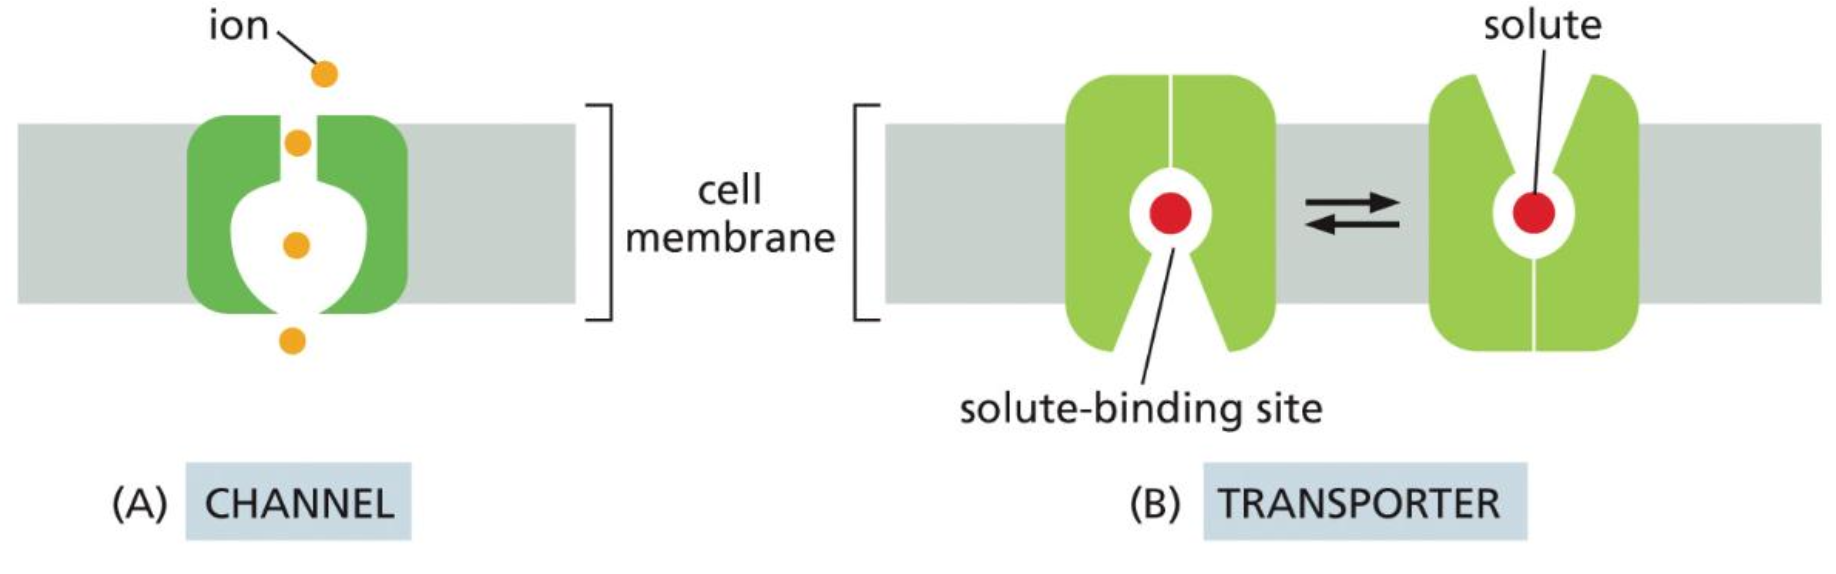
\includegraphics[width=35mm]{src/Images/channel.png}
\end{minipage}
\begin{minipage}{0.58 \linewidth}
    \begin{itemize}
        \item selective to size and charge of solute
        \item bidirectional
        \item gated by external inputs
        \item Transporter good for large molecules
    \end{itemize}
\end{minipage}
\begin{minipage}{0.45\linewidth}
\subsection*{Active Transport}
\textbf{Pumps:}\\
    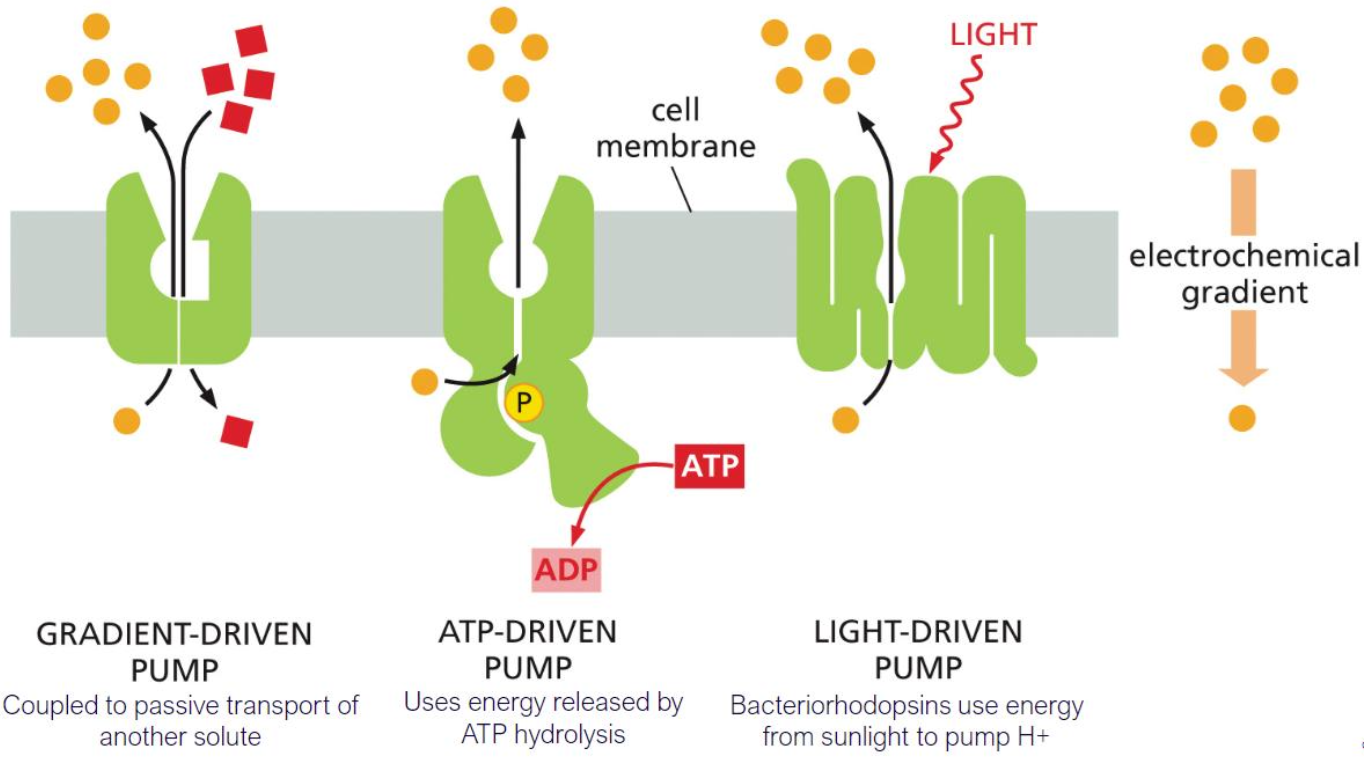
\includegraphics[width=35mm]{src/Images/pumps.png}

\end{minipage}
\vline \hspace{1mm}
\begin{minipage}{0.5\linewidth}
\subsection*{Vesicular Transport}
\textbf{Endocytosis:} into cell\\
\textbf{Exocytosis:} out of cell\\
\textbf{Pinocytosis:} cell drinking\\
\textbf{Phagocytosis:} cell eating\\
\textbf{Receptor-mediated endocytosis:} specific uptake of molecules\\

\vspace{5mm}
\end{minipage}
\subsection*{Intracellular Transport}
\begin{minipage}{0.41\linewidth}
    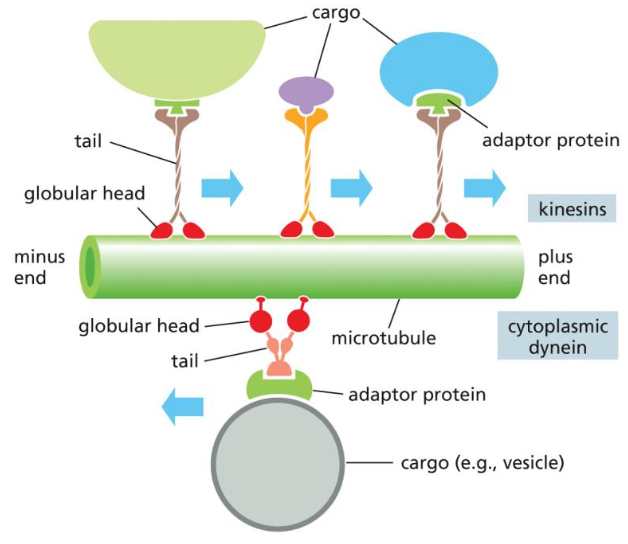
\includegraphics[width=35mm]{src/Images/intracellular.png}
\end{minipage}
\begin{minipage}{0.59\linewidth}
    \begin{itemize}
        \item chemical energy (ATP) to mechanical work
        \item directed motion
        \item Kinesin: carry out microtubule-based tiretrograde transport (towards cell edge)
        \item Dynein: carry out retrograde transport
(towards cell nucleus)
    \end{itemize}
\end{minipage}

\section*{Cell Sensing and Signaling}
\subsection*{Cellular Communication}
\textbf{Long Range:}\\
\begin{minipage}{0.5\linewidth}
    Endocrine
    \begin{itemize}
        \item into blood stream
        \item affect whole organism
    \end{itemize}
\end{minipage}
\begin{minipage}{0.5\linewidth}
    Neural
    \begin{itemize}
        \item in neurons (electric)
        \item at synapses (chemical)
    \end{itemize}
\end{minipage}
\\
\textbf{Short Range:}\\
\begin{minipage}{0.5\linewidth}
    Paracrine
    \begin{itemize}
        \item affect local tissue
    \end{itemize}
\end{minipage}
\begin{minipage}{0.5\linewidth}
    Contact Dependent
    \begin{itemize}
        \item direct binding 
    \end{itemize}
\end{minipage}
\subsection*{Signaling}
\textbf{Cell Surface Receptors:}\\
Extracellular signal molecule (hydrophilic or charged) causes receptor to releas intracellular signal molecule.\\

\textbf{Intracellular Receptors:}\\
Signal molecule (hydrophobic) cross the membrane and act inside the cell.\\

\textbf{Signal is:}\\
\begin{minipage}{0.3\linewidth}
    \begin{itemize}
        \item Amplified
        \item Integrated
    \end{itemize}
\end{minipage}
\begin{minipage}{0.6\linewidth}
    \begin{itemize}
        \item Distributed
        \item Modulated (feedback loop)
    \end{itemize}
\end{minipage}
\subsection*{Receptors}
\subsubsection*{Ion-channel-coupled \hspace{8mm} Enzyme-coupled}
\begin{minipage}{0.49\linewidth}
        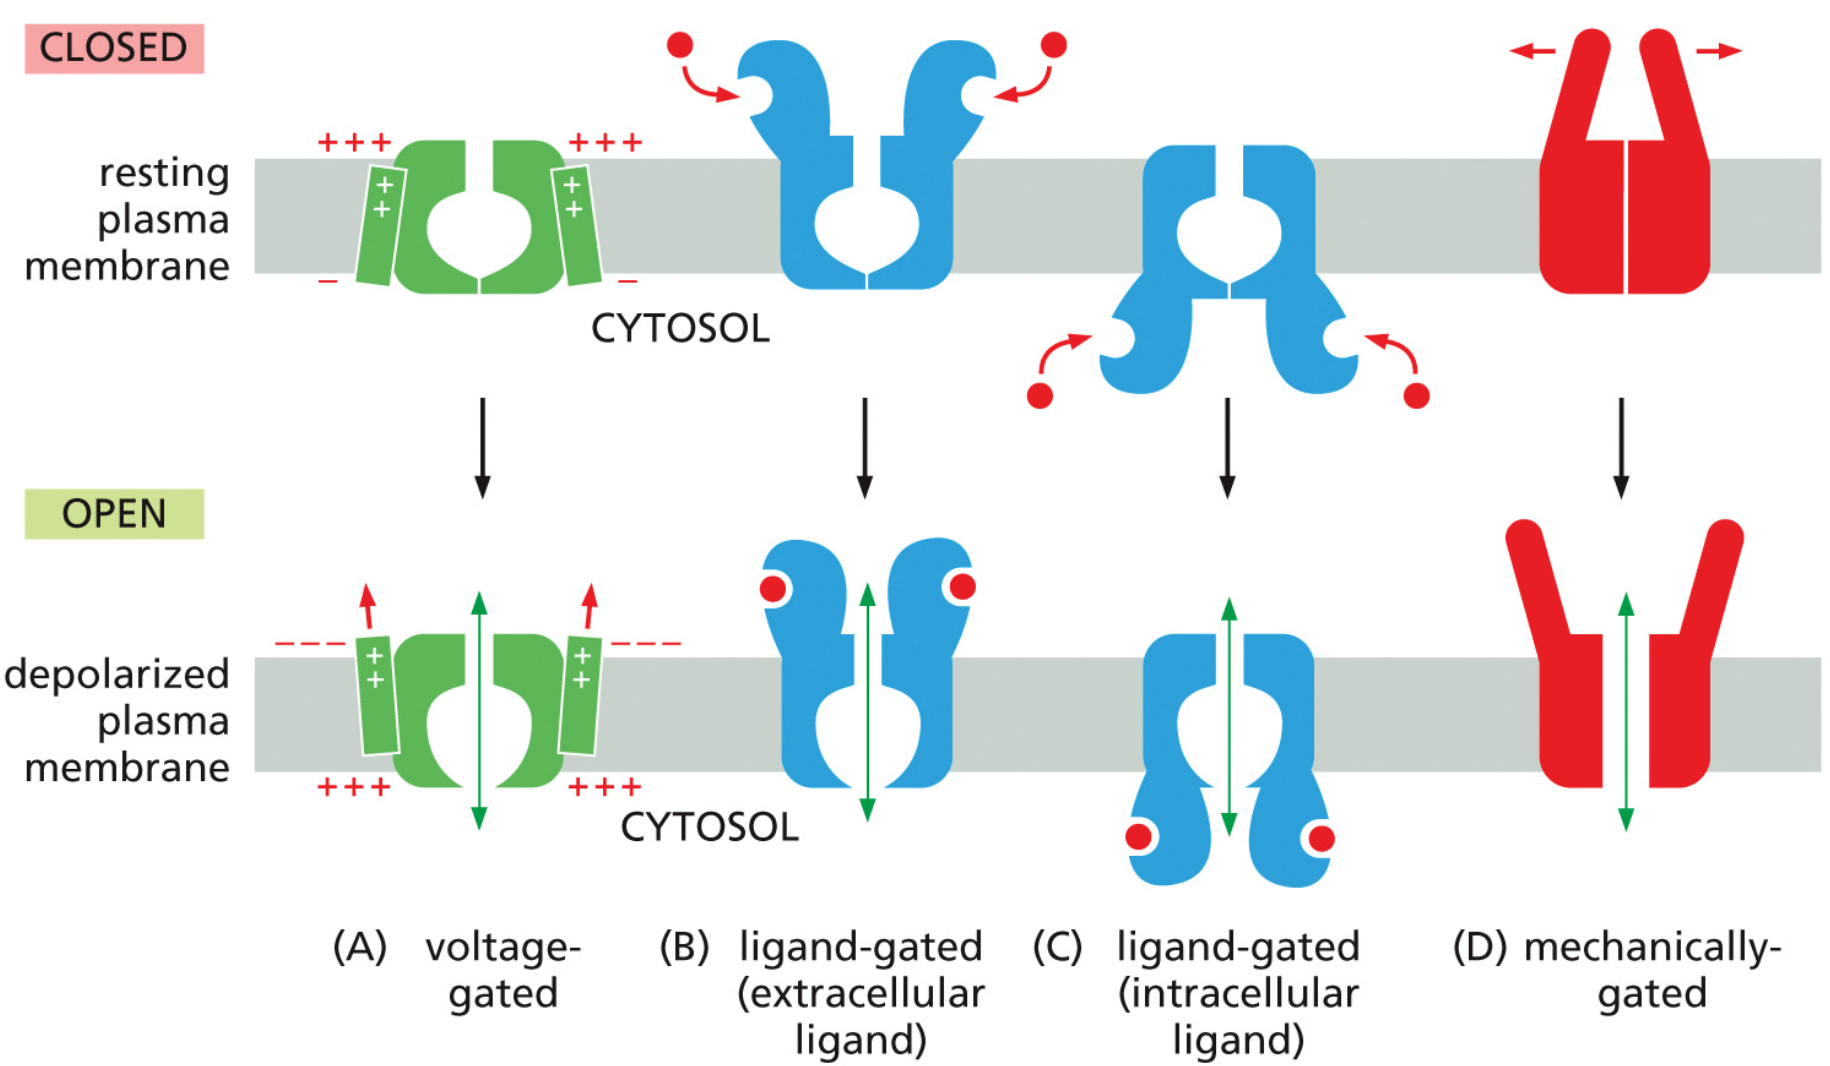
\includegraphics[width=28mm]{src/Images/ion_channel.png}
\end{minipage}
\begin{minipage}{0.49\linewidth}
    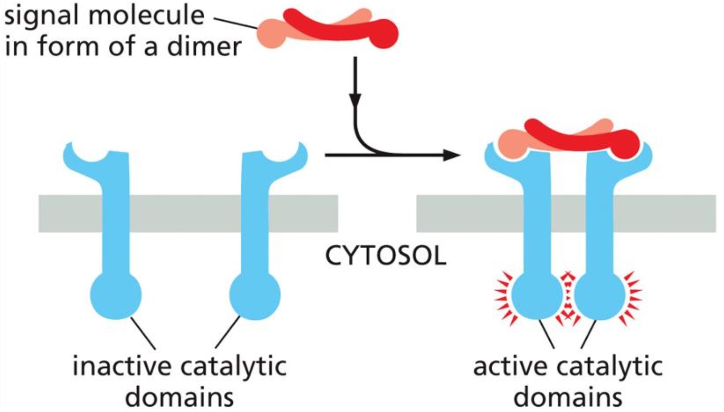
\includegraphics[width=28mm]{src/Images/enzyme_coupled.png}
\end{minipage}

\subsubsection*{G-protein-coupled receptors}
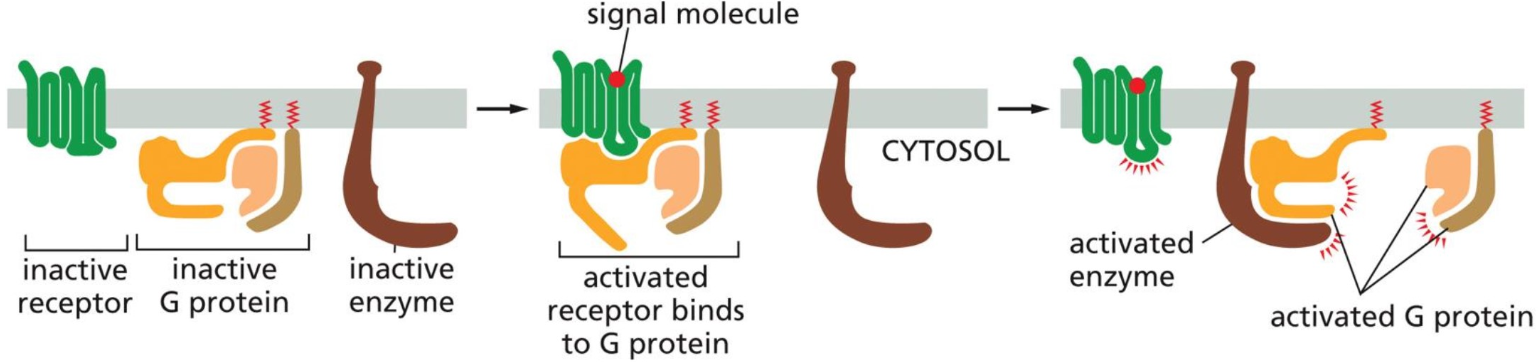
\includegraphics[width=70mm]{src/Images/g_protein.png}

\begin{itemize}
    \item Ligands (ex.: hormones, neurotransmitters) bind to GPCR (G-protein coupled receptor) which changes conformation
    \item Activated receptor causes G-protein to exchange its GDP for GTP gets activated
    \item G-protein modulates the activity of effector molecules generate intracellular second messenger
\end{itemize}


\vfill \null \columnbreak


\section*{Growth and Differentiation}
\subsection*{Cell Cycle}
\begin{minipage}{0.45\linewidth}
    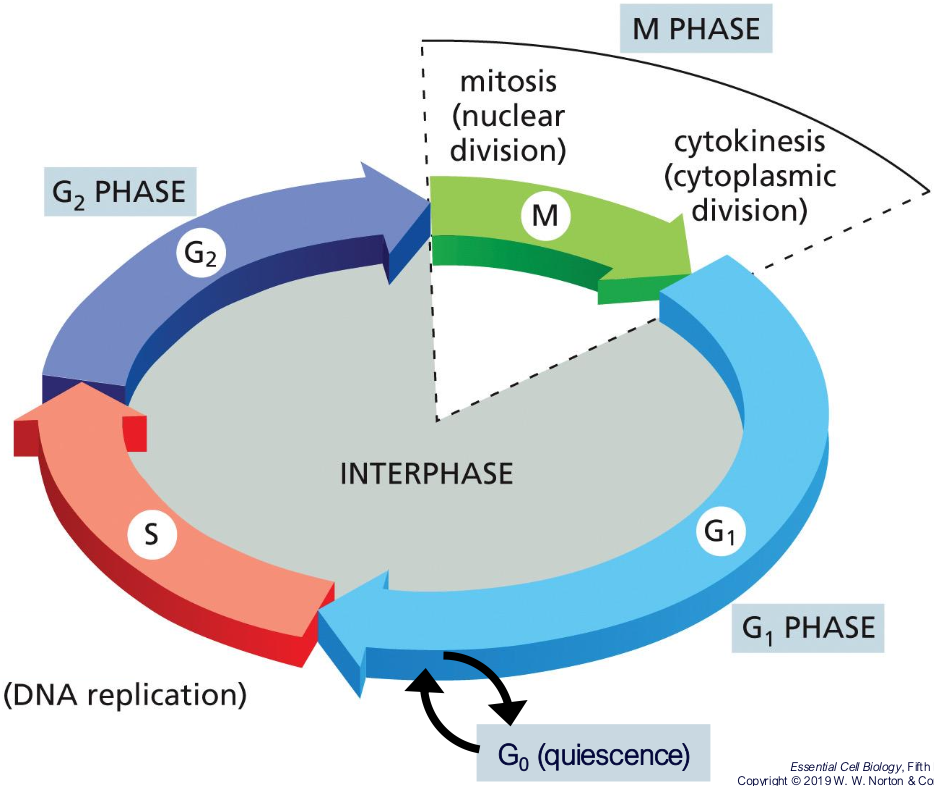
\includegraphics[width=30mm]{src/Images/cell_cycle.png}
\end{minipage}
\begin{minipage}{0.45\linewidth}
    \textbf{G1:} Cell growth \\
    \textbf{S:} DNA Synthesis \\
    \textbf{G2:} Growth and preparation for Mitosis \\
    \textbf{M:} Mitosis (cell division) \\
    Quiescent cells: cells pause before replication. Reversible growth arrest (G0 phase) \\
    Proliferation: populartion $\nearrow$ 
\end{minipage}
\subsection*{Growth}
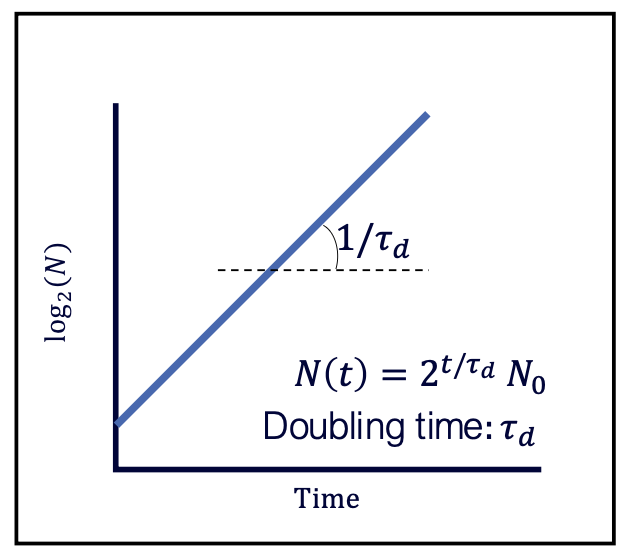
\includegraphics[width=23mm]{src/Images/doubling_time.png}
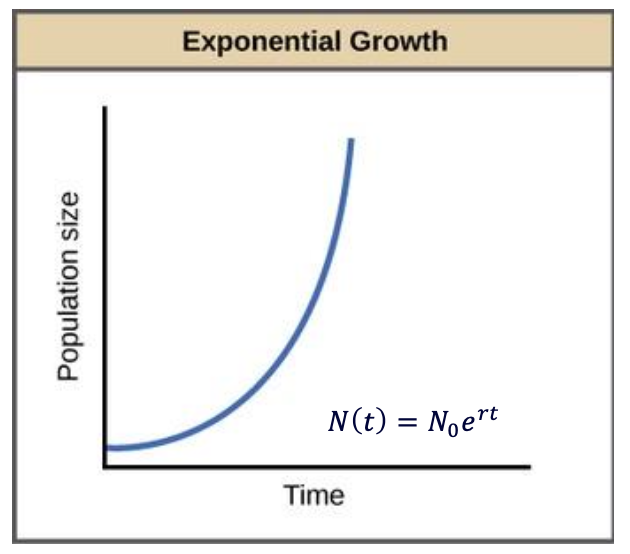
\includegraphics[width=23mm]{src/Images/exp_growth.png}
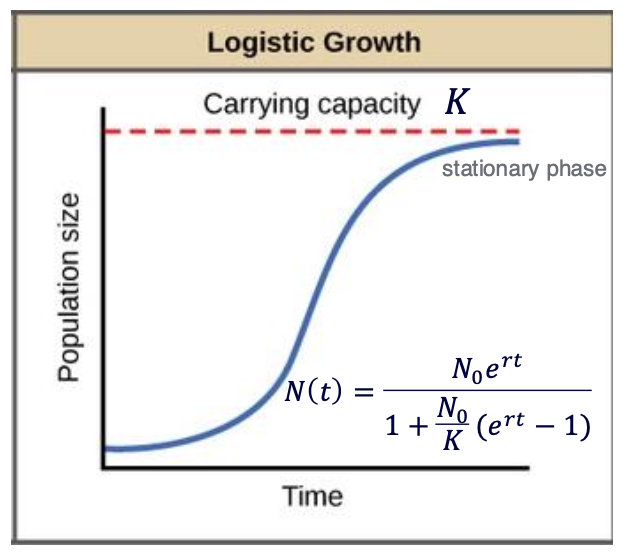
\includegraphics[width=23mm]{src/Images/log_growth.png}

\subsection*{Clonal Population}
\textbf{Genotype:}
ensemble of all the genes of a cell ("all available genes")\\
\textbf{Phenotype:}
output of set of expressed genes ("all visible genes")\\
\textbf{Clonal population:}
same genotype and phenotype, identical cells, 
can differ due to mutations in genotype

\subsection*{Cell Death}
\begin{minipage}{0.48\linewidth}
    \textbf{Apoptosis:}
        \begin{itemize}
            \item controlled cell death
            \item directed by extracellular signals
            \item controlled by intracellular signal cascade
            \item apoptotic cell gets phagocytosed by macrophages
        \end{itemize}
\end{minipage}
\begin{minipage}{0.45\linewidth}

    \textbf{Necrosis:}
        \begin{itemize}
            \item death as result of injury
            \item cells burst and release their contents
        \end{itemize}
        \vspace{16mm}
\end{minipage}
\subsection*{Stem Cells – Cell Differentiation}
\textbf{Differentiated cells} in adult organisms contain all the genetic information to form a new organism.
But, they express \textbf{only a fraction} of genes \textbf{specific to their function}.\\

Stem cells can differentiate to tissue-specific cell, but also renew themselves.\\

\textbf{Pluripotent stem cells} can give rise to all cell types.\\
\textbf{Multipotent stem cells} can give rise to a limited number of cell types tissue specific.\\

\section*{Bioprocesses}
Bioprocesses rely on several key components, including biological 
components, such as the \textbf{target molecule} and the \textbf{cells} used
to produce it; \textbf{culture medium} and one or more \textbf{bioreactors}; as well as a \textbf{process}.\\

Modern technology used:
    \begin{itemize}
        \item DNA sequencing and synthesis
        \item Precise gene editing
        \item Genetic circuit design
    \end{itemize}

\textbf{Cell source:} \\

\begin{minipage}{0.48\linewidth}
    Mammalian cells:
        \begin{minusitemize}
        \item slow growth
        \item complex growth media
    \end{minusitemize}
    \begin{plusitemize}
        \item proper folding
        \item glycosylation
    \end{plusitemize}
\end{minipage}
\begin{minipage}{0.45\linewidth}
    E. coli:
    \begin{plusitemize}
        \item fast
        \item simple growth media
    \end{plusitemize}
    \begin{minusitemize}
        \item refolding required
        \item no glycosylation
    \end{minusitemize}
\end{minipage}
\vspace{2mm}

\subsection*{Transfection}
\begin{minipage}{0.50\linewidth}
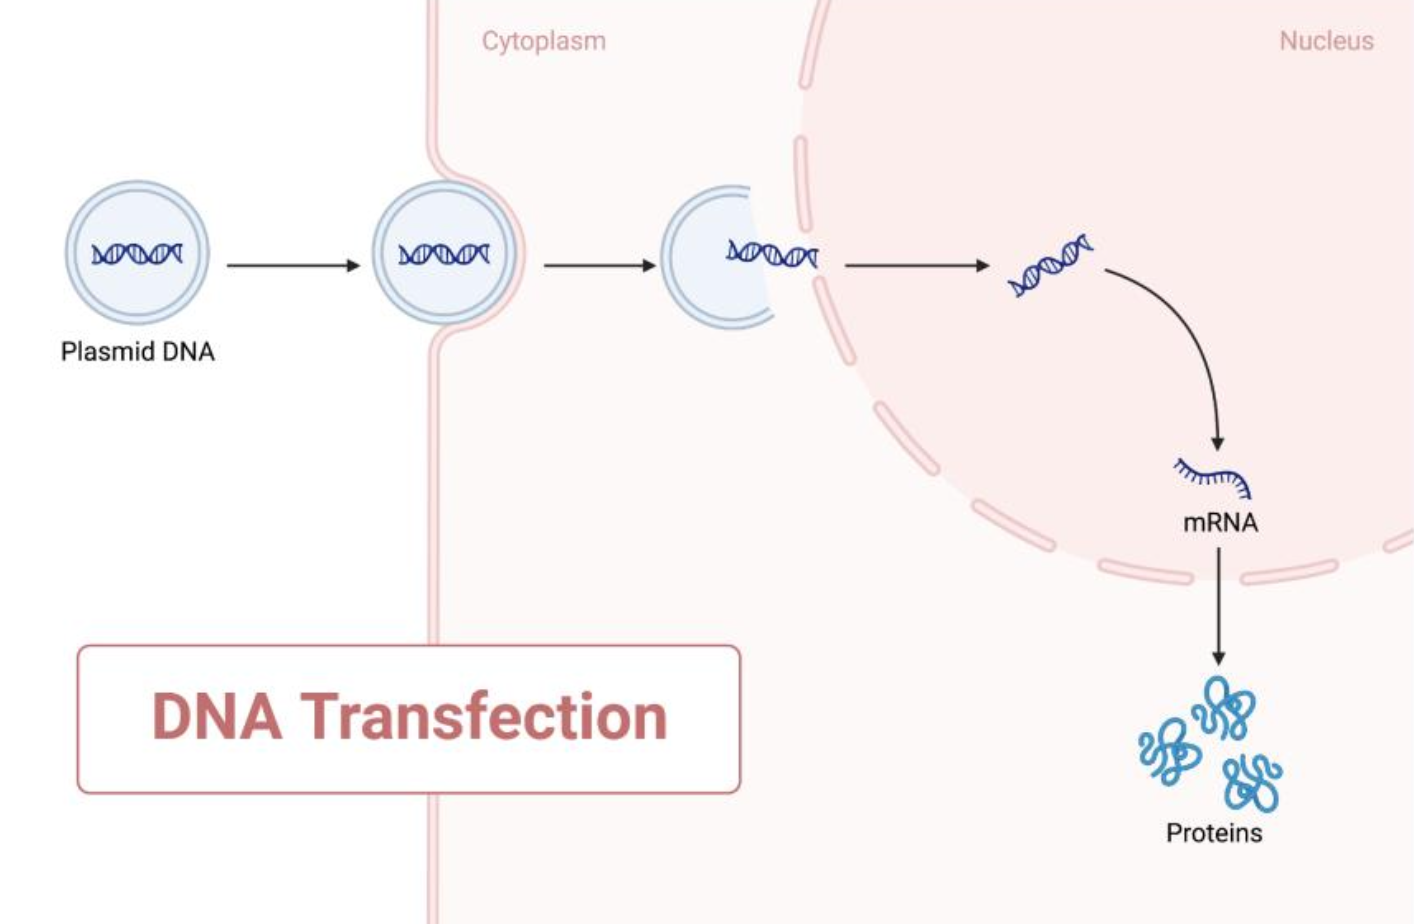
\includegraphics[width=35mm]{src/Images/transfection.png}
\end{minipage}
\begin{minipage}{0.45\linewidth}
    Insert DNA that codes for the wanted biomolecule into cell. Use:
    \begin{itemize}
        \item viruses
        \item electroporation
        \item carriers
    \end{itemize}
    store transfected cells in cryogenic conditions
\end{minipage}




\subsection*{4 Culture medium}
Source of nutrients to support the growth of cells. \\
Composition:
\begin{itemize} 
    \item building blocks (sugars, aa)
    \item water
    \item salts/ions
\end{itemize}

\subsection*{5 Bioreactor}
Carefully designed \textbf{culture medium} that
\textbf{provides nutrients} (building blocks,
water, ions, energy) and a \textbf{suitable
environmen} for cells to grow and
generate biomolecules of interest.\\

\begin{minipage}{0.45\linewidth}
    Batch
    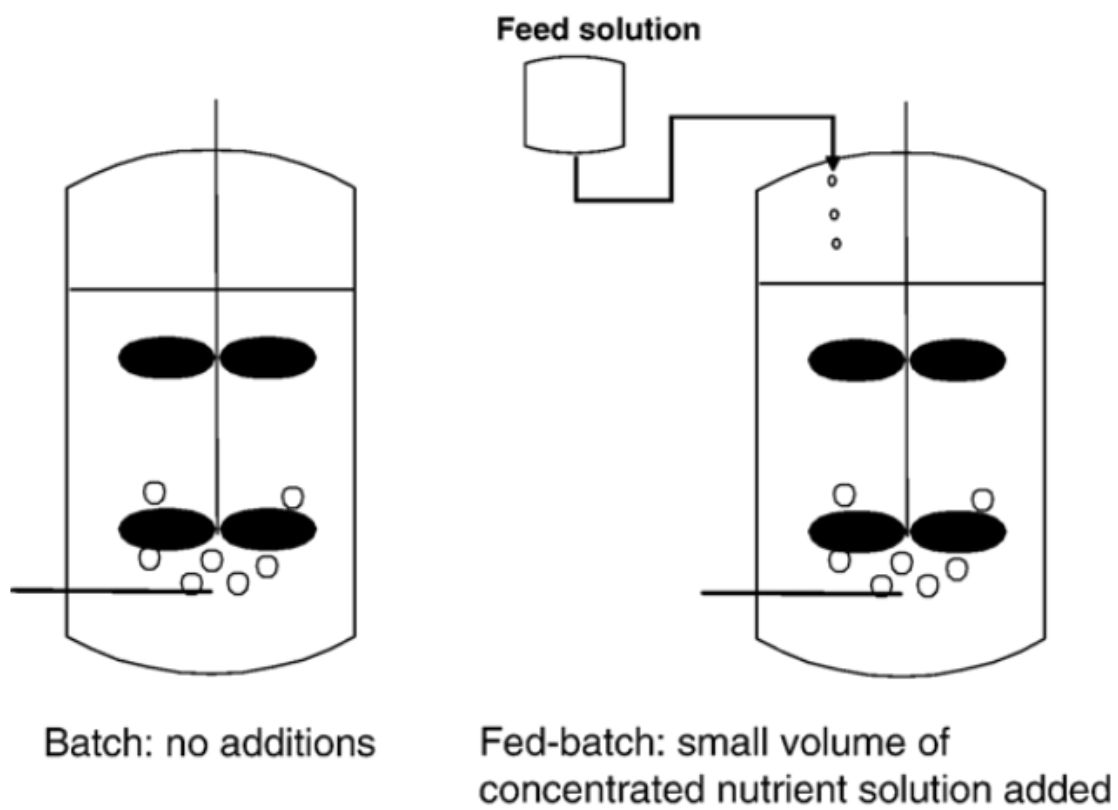
\includegraphics[width=33mm]{src/Images/batch.png}
\end{minipage}
\begin{minipage}{0.45\linewidth}
    Perfusion
    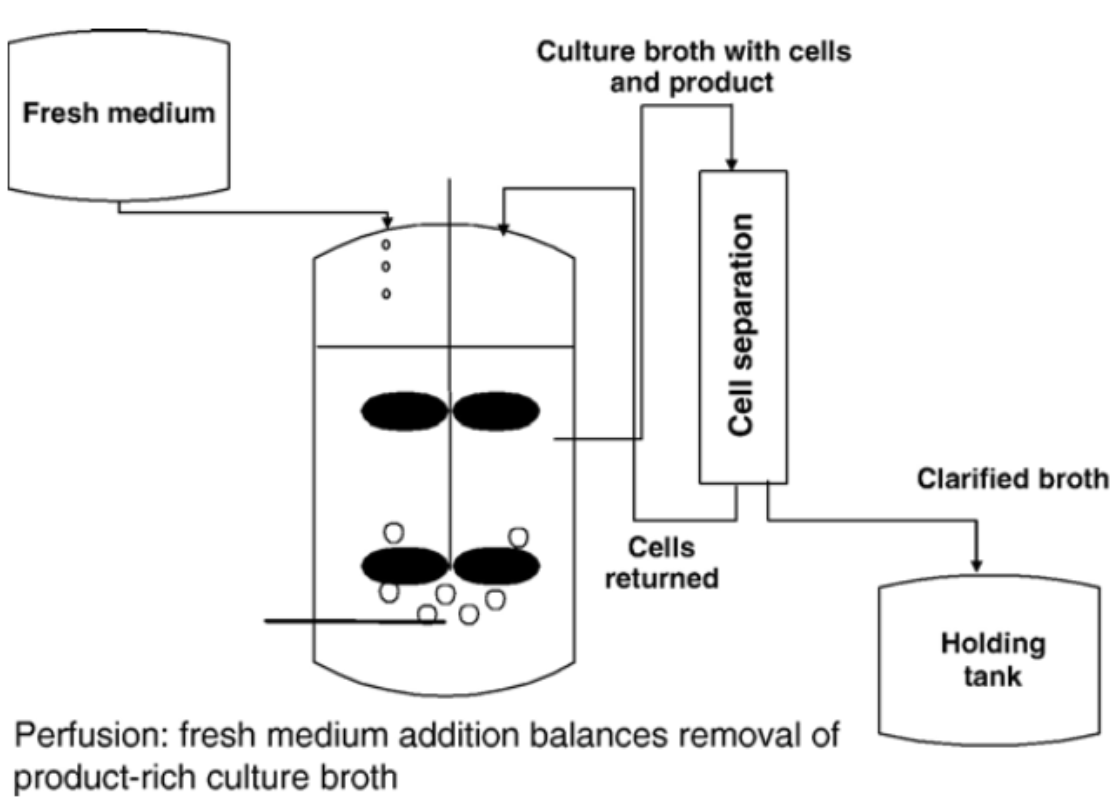
\includegraphics[width=33mm]{src/Images/perfusion.png}
\end{minipage}

% \section*{Cell and tissue architecture}

% \section*{Woundhealing and Tissue Engineering}

% \section*{Microphysiological Systems and Immune Engineering}

% \section*{Foodprocessing}

% \section*{Drug Delivery}








\end{document}